\documentclass[11pt, titlepage]{article}

\usepackage{amsmath, graphicx}

\begin{document}


\author{Antoine Lefebvre}
\title{Burning analysis of star configuration}
\maketitle

\tableofcontents 

\newpage

\section{Introduction}

The design of solid propellant grain that provide neutral burning
is important to optimize rocket motor performance. The star
configuration have been widely used to achieve this goal. In this
report, I will present an analysis of the burning comportement of star
shape as well as parameter recommandation to achieve better
performance.

\section{Geometric definition}

The star could be characterize by seven independant variable as
defined in figure \ref{star}. As every star points are identical,
only one is necessary for the analysis. 

\begin{figure}
 \begin{center}
 \includegraphics[height=5in]{img/variable.ps}
      \caption{Geometric definition of star.}\label{variable}
 \end{center}
\end{figure}

\begin{align*}
   w &= \text{Web thickness}\\
 r_1 &= \text{Radius}\\
 r_2 &= \text{Tip radius}\\
   R &= \text{External radius}\\
\eta &= \text{angle}\\
\varepsilon &= \text{Secant fillet angle}\\
   N &= \text{Number of star points}\\
%S &= \text{burning perimeter as a function of } wx\\
\end{align*}


\begin{figure}
 \begin{center}
 \includegraphics[height=4in]{img/mainstar.ps}
      \caption{Burning zone of the star configuration.}\label{star}
 \end{center}
\end{figure}

\section{Analysis}

In this section, an expression for the perimeter of the star will be
developp for each burning zone as a function of the web thickness
burned ($w_x$).

  \subsection{Zone 1}
  
  The perimeter in the zone one could be divide in three
  sections. Starting by the right, we have the section before the
  radius $r_1$, which have a radius equal to $R-w+w_x$. The length of
  this section is then: $(R-w+w_x)(\pi/N - \varepsilon)$.

  Then, we have the perimeter of the arc of initial radius $r_1$. The
  angle will remain constant to $a$. The length is then: $(r_1+w_x)a$.

  The third section is more complicated. The lenght of the line
  starting at the end of the radius $r_1$ and crossing the vertical
  line will be evaluated first. Then, the perimeter of the radius
  $r_2$ will be add to the result, and the length of the line starting
  at the beginning of the radius will be substract.

\begin{figure}
 \begin{center}
 \includegraphics[height=5in]{img/starL.ps}
      \caption{Determination of the length $L$.}\label{len}
 \end{center}
\end{figure}

  In order to determine the length, refer to the figure \ref{len}. The
  lenght $L$ we are looking for will be equal $x + y$.

\begin{align*}
     b + z &= (R-w-r_1)\sin{\varepsilon}\\
         x &= (r_1+w_x)\tan{\eta}\\
\cos{\eta} &= \frac{r_1+w_x}{z}\\
\sin{\eta} &= \frac{b}{y}\\
\sin{\eta} &= \frac{(R-w-r_1)\sin{\varepsilon} -
    \frac{r_1+w_x}{\cos{\eta}}}{y}\\
 L = y + x &= (R-w-r_1)\frac{\sin{\varepsilon}}{\sin{\eta}} - 
              \frac{r_1+w_x}{\cos{\eta}\sin{\eta}} +
              (r_1+w_x)\tan{\eta}
\end{align*}

  We could now simplify this equation using two trigonometric
  identity:

\begin{align*}
  \sin^2{\eta} -1 &= -\cos^2{\eta}\\
       \tan{\eta} &= \frac{1}{\tan{(\frac{\pi}{2}-\eta)}}
\end{align*}

\begin{equation}
\begin{split}
  L &= (R-w-r_1)\frac{\sin{\varepsilon}}{\sin{\eta}} + 
             (r_1+w_x)\left[
             \frac{\sin^2{\eta}-1}{\cos{\eta}\sin{\eta}} \right]\\
      &= (R-w-r_1)\frac{\sin{\varepsilon}}{\sin{\eta}} + 
             (r_1+w_x)\left[ \frac{-\cos{\eta}}{\sin{\eta}} \right]\\
      &= (R-w-r_1)\frac{\sin{\varepsilon}}{\sin{\eta}} + 
             (r_1+w_x)\left[ \frac{-1}{\tan{\eta}} \right]\\
      &= (R-w-r_1)\frac{\sin{\varepsilon}}{\sin{\eta}} - 
             (r_1+w_x)\tan{(\frac{\pi}{2}-\eta)}\\
\end{split}
\end{equation}


 We could now determine the length of the arc and how much we should
 substract from the length L. Refer to figure \ref{arc} for the
 variables.

 \begin{figure}
 \begin{center}
 \includegraphics[height=3in]{img/arc.ps}
      \caption{Arc of radius $r_2$.}\label{arc}
 \end{center}
\end{figure}

  $$\text{Arc length} = (r_2-wx)(\frac{\pi}{2}-\eta)$$

  $$x = \frac{r_2-wx}{\tan{\eta}}$$

 We have now the complete expression of the perimeter of the star as a
 function of web burned ($w_x$) in the zone one. This expression is
 valid for $0 < w_x < r_2$.

\begin{equation}
  \begin{split}
  \frac{S}{2N} &= (R-w+w_x)(\frac{\pi}{N} - \varepsilon) +
                  (r_1+w_x)a+(R-w-r_1)\frac{\sin{\varepsilon}}{\sin{\eta}}\\ 
               & \quad - (r_1+w_x)\tan{(\frac{\pi}{2}-\eta)}
               + (r_2-w_x)(\frac{\pi}{2}-\eta) \\
               & \quad - (r_2-wx)\tan{(\frac{\pi}{2}-\eta)}\\
               &= (R-w+w_x)(\frac{\pi}{N} - \varepsilon) +
                  (r_1+w_x)a+(R-w-r_1)\frac{\sin{\varepsilon}}{\sin{\eta}}\\ 
               & \quad - (r_1+r_2)\tan{(\frac{\pi}{2}-\eta)}
               + (r_2-w_x)(\frac{\pi}{2}-\eta)\\
  \end{split}
\end{equation}


  We could now determined the first derivative of this expression to
  evaluate if it is progressive, regressive or neutral.

  \begin{equation}
  \frac{\delta S}{\delta w_x} = 2N\left[ \frac{\pi}{N} - \varepsilon + a -
  \frac{\pi}{2} + \eta \right]
  \end{equation}

  We could verify that:

  $$a = \frac{\pi}{2} - \eta + \varepsilon$$

  Our expression become:

  \begin{equation}
  \frac{\delta S}{\delta w_x} = 2\pi
  \end{equation}

  
  The perimeter in zone 1 will always be progressive. So, it is
  important to minimize the radius $r_2$ in order to switch as fast as
  possible to the zone 2.


  \subsection{Zone 2}
  
  The expression for the perimeter in the second zone is almost the
  same as in the zone one. The difference is that the radius $r_2$ had
  vanish and the expression reduce to a simpler one:

\begin{equation}
 \begin{split}
  \frac{S}{2N} &= (R-w+w_x)(\frac{\pi}{N} - \varepsilon) +
                 (r_1+w_x)a+(R-w-r_1)\frac{\sin{\varepsilon}}{\sin{\eta}}\\ 
               & \quad - (r_1+w_x)\tan{(\frac{\pi}{2}-\eta)}\\
 \end{split}
\end{equation}

  The derivative of this expression is:

 \begin{equation}
  \begin{split}
   \frac{\delta S}{\delta w_x} &= 2N\left[ \frac{\pi}{N} -\varepsilon +
                                  a - \tan{(\frac{\pi}{2} - \eta)} \right]\\
                               &= 2N\left[ \frac{\pi}{2} - \eta +
                                  \frac{\pi}{N} - \tan{(\frac{\pi}{2}
                                  - \eta)} \right]\\
  \end{split}  
 \end{equation}

  As we could see in this expression, the progressivity in zone 2 is
  determined by the angle $\eta$ and by the number of star point
  $N$. It is independant of the angle $\varepsilon$.

  The zone 2 will be predominant during the motor burn time and we
  would like to provide neutrallity in this zone. Neutrality is obtain
  when the derivative of the perimeter is equal to zero. This lead to
  the following equation:

\begin{equation}
  \frac{\delta S}{\delta w_x} = 0 = \frac{\pi}{2} - \eta +
                                   \frac{\pi}{N} - \tan{(\frac{\pi}{2}
                                   - \eta)}
\end{equation}

  Which reduce to the following implicit equation of $\eta$ as a
  function of $N$:


\begin{equation}
\eta = \frac{\pi}{N} - \tan{(\frac{\pi}{2} - \eta)} + \frac{\pi}{2}
\end{equation}

  Solution of this equation give values of the angle $\eta$ to obtain
  neutrality in zone 2 as a function of the number of star points.

\begin{center}
 \begin{tabular}{||c|c|c||}
  \hline
  \hline
  $N$ & $\eta$ (deg) & $\pi/N$ (deg) \\
  \hline
  3 & 24.55 & 60.00\\
  4 & 28.22 & 45.00\\
  5 & 31.13 & 36.00\\
  6 & 33.53 & 30.00\\
  7 & 35.56 & 25.71\\
  8 & 37.31 & 22.50\\
  9 & 38.84 & 20.00\\
  \hline
 \end{tabular}
\end{center}
  
  It is important to note that when the angle $\eta < \pi/N$, a secant
  fillet $\varepsilon < \pi/N$ will be necessary to prevent star point
  from overlapping. In general, $\varepsilon$ should always be smaller
  that $\pi/N$.
                 
  \subsection{Zone 3}

  The perimeter in the zone 3 begin when $w_x = Y*$. The angle $a$
  become progressivly smaller when propellant burned. Perimeter could
  be expressed like this:

\begin{equation}
\frac{S}{2N} = (R-w+w_x)(\frac{\pi}{N}-\varepsilon) + 
               (r_1+w_x)\left[ \varepsilon +
               \arcsin{(\frac{R-w-r_1}{r_1+w_x}\sin{\varepsilon}}) \right]
\end{equation}


  The derivative of this expression become:

\begin{equation}
\begin{split}
\frac{\delta S}{\delta w_x} &= 2N \biggl[ \frac{\pi}{N}  +
       \arcsin{\biggl(\frac{R-w-r_1}{r_1+w_x}\sin{\varepsilon}\biggr)} - \\
      &\quad  \frac{w_x(R-w-r_1)\sin{\varepsilon}}{(r_1+w_x)^2\sqrt{1-\frac{(R-w-r_1)^2\sin^2{\varepsilon}}{(r_1+w_x)^2}}} \biggr]\\
\end{split}
\end{equation}


  It could be demonstrate that the perimeter is progressive in this
  section. It would be interesting to eliminate the zone 3 in order to
  keep neutrality as long as possible.

  The condition for the elimination of zone 3 is:

\begin{equation}
  Y* = (R-w-r_1)\frac{\sin{\varepsilon}}{\cos{\eta}} - r_1 = w
\end{equation}

  This equation reduce to:

\begin{equation}
  \sin{\varepsilon} = \frac{w+r_1}{R-w-r_1}\cos{\eta}
\end{equation}

  Now, the angle $\varepsilon$ is determine by the web thickness $w$,
  the radius $r_1$ and the angle $\eta$. As $\eta$ was determine by
  the number of star points $N$ and the radius may be dictate by
  technical decision, the web thickness $w$ will determine
  $\varepsilon$.

  \subsection{Zone 4}

  The analytical solution of the perimeter in the zone 4 could be
  found with the help of the cosinus law:

\begin{equation*}
 c^2 = a^2 + b^2 - 2ab\cos{\theta}
\end{equation*}

  The perimeter is then:
\begin{equation}
\begin{split}
\frac{S}{2N} = (r_1+w_x) \biggl[ & \varepsilon +
      \arcsin{\biggl(\frac{R-w-r_1}{r_1+w_x}\sin{\varepsilon}\biggr)}
      - \pi\\
      & \quad + \arccos{\biggl(\frac{(r_1+w_x)^2+(R-r_1-w)^2-R^2}{2(r_1+w_x)(R-r_1-w)}\biggr)}
      \biggr]\\
\end{split}
\end{equation}



\section{Design example}

  In this section, a star configuration will be design with the
  theory developp in the previous sections for a motor of $3 inch$
  internal diameter.

  The goal is to have a perimeter that will remain as constant as
  possible to mainatin neutrality. It will also be interesting to
  minimize the number of star points in order to reduce the difficulty
  to cast the propellant. We could also try to optimize the volumetric
  loading.

%  \subsection{Solution}

  First of all, we could determine the number of star points. In order
  to maximize the quantity of matter, the angle $\varepsilon$ should
  be equal to $\pi/N$. In order to obtain this condition, the angle
  $\eta$ should be larger than $\pi/N$. 

  If we refer to the table of the angle $\eta$ in function of $N$, to
  obtain neutrality in zone 2, we must choose $N=6$ to have $\eta >
  \pi/N$.

  Three conditions are now determine:

$$N = 6$$
$$\eta = 33.53 deg$$
$$\varepsilon = 30 deg$$

  We must now found the web thickness $w$ and radius $r_1$ that fit
  the conditions. A radius $r_1 = 1/16 in$ is reasonable technically.

  The equation to be solve is the following:

$$sin{\varepsilon} = \frac{w+r_1}{R-w-r_1}\cos{\eta}$$

  The value of $w$ that solve this equation is:

$$w = 0.500$$

  The seven independant variable are now fixed. The resulting shape
  could be seen in figure \ref{res}.


\begin{figure}
 \begin{center}
 \includegraphics[]{img/res.ps}
      \caption{Resulting star configuration for the 3 inch motor.}\label{res}
 \end{center}
\end{figure}


  With the functions developp in the report, the evolution of the
  perimeter as a function of the web burned could be plot.

\begin{figure}
 \begin{center}
 \includegraphics[height=4in]{img/perimeter.ps}
      \caption{Graphic of the perimeter as a function of web burned.}\label{grah}
 \end{center}
\end{figure}


\section{conclusion}

The star configuration offer the possibility to design rocket motor
that works at almost constant pressure. It is then possible to
optimize on case thickness and throat diameter in order to obtain the best
performance.

\begin{thebibliography}{}
\bibitem{nasa} NASA SP-8076, {\em Solid Propellant Grain Design And
Internal Ballistics}, March 1972
\end{thebibliography}

\end{document}









